% =========================================================================
% Main LaTeX Document for Springer Computer Science Proceedings (LNCS)
% Formatted strictly according to Springer Author Guidelines (reference.pdf)
% =========================================================================

\documentclass{llncs}

% -------------------------------------------------------------------------
% 1. Character Encoding & Fonts
% -------------------------------------------------------------------------
\usepackage[T1]{fontenc}
\usepackage[utf8]{inputenc}

% Springer LNCS recommended font settings (Times Roman based)
\usepackage{newtxtext}
\usepackage[varvw]{newtxmath}

% -------------------------------------------------------------------------
% 2. Figures & Graphics
% -------------------------------------------------------------------------
\usepackage{graphicx}
% Set search path for graphic files (e.g., pdf, eps, png)
\graphicspath{{./figures/}{./}}

% -------------------------------------------------------------------------
% 3. Tables & Formatting
% -------------------------------------------------------------------------
\usepackage{booktabs}       % High-quality academic tables (avoid vertical lines)
\usepackage{multirow}       % Multirow cells in tables
\usepackage{array}          % Advanced column configurations

% -------------------------------------------------------------------------
% 4. Microtypography & Symbols
% -------------------------------------------------------------------------
\usepackage{microtype}      % Improves spacing and reduces overfull hboxes
\usepackage{bbding}         % Provides \Envelope for corresponding author marking

% -------------------------------------------------------------------------
% 5. Hyperlinks & URLs (Springer eBook style)
% -------------------------------------------------------------------------
\usepackage{xcolor}
\usepackage{hyperref}
\hypersetup{
    colorlinks=true,
    linkcolor=blue,
    citecolor=blue,
    urlcolor=blue,
    pdfstartview={FitH}
}
% Springer guidelines: URLs displayed in blue roman font
\renewcommand\UrlFont{\color{blue}\rmfamily}
\urlstyle{rm}

% =========================================================================
% Front Matter
% =========================================================================
\begin{document}

% --- Title ---
% Guideline: Capitalize nouns, verbs, and all other words except articles,
% prepositions, and conjunctions (Title Case).
\title{Do Students Agree with LLM Feedback on Their Own Code? A Within-Subject Study of Four Feedback Configurations in Software Project Courses}

% Running heads are disabled (uncomment if required later for camera-ready):
%\titlerunning{Do Students Agree with LLM Feedback on Their Own Code?}

% --- Authors ---
% Guideline:
% - Full given name before surname.
% - Mark the corresponding author with (\Envelope).
\author{
    Phuc Sanh Nguyen \and
    Song Huong Dang \and
    Quang Hieu Le \and
    Viet Bao Nguyen \and
    \mbox{Phuc Thinh Do(\Envelope)}
}

%\authorrunning{P. S. Nguyen et al.}

% --- Affiliation & Emails ---
\institute{
    FPT University, Ho Chi Minh City, Vietnam\\
    \email{npsdn1906@gmail.com, dangsonghuong010405@gmail.com,\\
    lequanghieu2504@gmail.com, babluokei4@gmail.com, ThinhDP2@fe.edu.vn}
}

\maketitle % Typeset title, authors, affiliations

% =========================================================================
% Abstract & Keywords
% =========================================================================
\begin{abstract}
Oral defense (viva) in software engineering capstone projects is essential for verifying students' comprehension of business logic and codebase architecture, yet manual grading is labor-intensive and inconsistent, whereas off-the-shelf large language models (LLMs) risk code-context hallucinations, prompt injection, and sycophantic grading. This paper presents the pedagogical evaluation and feedback engine of \textbf{PACE}, an AI-assisted viva assessment system combining complexity-aware hybrid ground-truth extraction (routing raw source code versus Mermaid control/data-flow graphs at a function-node threshold of $\tau = 10$) with a three-layer safety guardrail architecture and XML-based delimiter sandboxing. To mitigate single-model grading sycophancy, we propose a role-decoupled \textbf{Multi-LLM Ensemble} (\textit{Researching} mode) sequentially chaining \textbf{DeepSeek-V3} (\textit{Code Inspector}) with \textbf{Groq (\texttt{openai/gpt-oss-120b})} (\textit{Pedagogical Synthesizer and Rubric Grader}), evaluated alongside three single-LLM formative feedback formats (\textit{Sandwich}, \textit{Rubric}, and \textit{Explainable}). In a randomized, student-blinded, within-subject experiment at FPT University, 86 students across 28 capstone repositories submitted 344 scenario-based viva responses ($k = 4$ per student) and rated each feedback instance using a 15-item, five-point Likert-scale instrument with unidirectional positive keying, adapted from the Feedback Perceptions Questionnaire (FPQ), explainable AI (XAI), argument persuasiveness, psychological safety, and TAM/UTAUT frameworks. Across 344 ratings, the proportions of positive student responses (ratings of 4 or 5 out of 5) endorsed AI judgment (\texttt{ACCEPTANCE}: 79.9\%), future use intention (\texttt{BEHAVIORAL INTENTION}: 68.0\%), and learning-related encouragement and self-reported motivation (\texttt{AFFECT}: 41.9\%), yielding an overall multidomain composite mean of 4.07/5 (95\% CI [3.90, 4.23]). All six repository-level 95\% bootstrap confidence intervals for direct acceptance (\texttt{ACCEPTANCE}) included zero without establishing statistical equivalence, and observational raw-versus-graph acceptance remained inconclusive ($b = 0.03$, 95\% CI [$-0.18$, 0.26]). Exploratory analysis revealed a 0.37-point actionability (\texttt{ACTIONABILITY}) difference between \textit{Sandwich} and \textit{Explainable} (approximate simultaneous 95\% sensitivity interval [0.02, 0.72] across 90 paired item-level contrasts derived from 6 format pairs $\times$ 15 criteria) without isolating the independent effect of the \texttt{next\_steps} component. These findings reflect learners' self-reported perceptions rather than expert-verified accuracy, actual revision behavior, or learning gains.

\keywords{Automated Viva Assessment \and Multi-LLM Ensemble \and Formative Feedback \and Pedagogical AI Guardrails \and Software Engineering Education.}
\end{abstract}

% =========================================================================
% Main Content
% =========================================================================

\section{Introduction}
\label{sec:intro}

Formative feedback is widely recognized as an important factor in improving student learning. However, its effectiveness depends largely on how learners understand, interpret, and act on the guidance they receive~\cite{hattie2007power,shute2008focus}. Technically accurate feedback does not necessarily lead to better understanding or meaningful revisions~\cite{carless2018feedback,winstone2017supporting}. Research on feedback literacy emphasizes that students need to interpret feedback, make judgments about their own work, and use the feedback to guide their actions. These activities are essential parts of the feedback process, rather than simply outcomes that occur after feedback is provided~\cite{carless2018feedback,winstone2017supporting}. In human-computer interaction, users' acceptance of automated feedback and willingness to act on it are also influenced by its perceived usefulness~\cite{davis1989perceived,venkatesh2003user}, as well as by psychological factors such as trust and users' tendency to accept or reject algorithmic judgments~\cite{lee2004trust,dietvorst2015algorithm,logg2019algorithm}.

With the rapid development of generative artificial intelligence, large language models (LLMs) are increasingly used in computing education to identify code issues and provide formative feedback at scale~\cite{kasneci2023chatgpt,denny2024computing,dai2023can}. However, general-purpose LLMs may generate inaccurate feedback when they lack sufficient context about the actual student codebase, including cases in which they misinterpret code or produce unsupported explanations~\cite{hellas2023exploring,kiesler2023exploring}. In addition, deploying LLMs in educational assessment requires appropriate safeguards to maintain pedagogical boundaries and reduce the risk of misuse, including prompt injection attacks~\cite{liffiton2023codehelp}. Recent studies in programming education and higher education have also found that students' perceptions of AI-generated feedback vary across several dimensions, including technical accuracy, level of detail, the availability of supporting evidence, and trust in comparison with feedback from human experts~\cite{escalante2023ai,zhang2024students,nazaretsky2024ai,er2025assessing}.

Two research gaps motivate this study:

\begin{itemize}
    \item \textbf{Gap 1 (Automated Viva Assessment and Hybrid Ground-Truth Contexts in Team Capstone Projects):}
    Software engineering capstone projects often involve shared codebases developed collaboratively by student teams. Traditional input-output autograders can assess whether a program produces the expected results, but they are less suited to determining whether individual students understand the code and its architecture. Although asking students questions about their own programs has been explored as a way to assess code understanding~\cite{lehtinen2021lets}, the use of automated, scenario-based oral defenses (viva) that combine multi-language static analysis with complexity-aware routing between different code representations remains underexplored.

    \item \textbf{Gap 2 (Formative Feedback Formats and Single-Model Sycophancy):}
    Using a single LLM as an automated evaluator (\textit{LLM-as-a-Judge}) can introduce biases, including a tendency to favor certain responses or follow patterns that affect grading consistency~\cite{zheng2023judging}. In practical systems, AI-generated feedback may combine praise, rubric-based assessment, code evidence, and model orchestration in different configurations. These configurations reflect different approaches to formative feedback: the \textit{Sandwich} format balances positive and corrective comments~\cite{parkes2013feedback}; \textit{Rubric} uses explicit scoring criteria to support consistent evaluation~\cite{jonsson2007use}; \textit{Explainable} emphasizes evidence and transparency~\cite{khosravi2022explainable}; and the \textit{Multi-LLM Ensemble} uses multiple models in coordinated roles to improve evaluation quality and reduce dependence on a single model's judgment~\cite{du2024improving,zheng2023judging}. However, comparative within-subject studies of these feedback formats, based on students' actual capstone project codebases and focused on learners' perceptions, remain limited.
\end{itemize}

To address these gaps, we present \textbf{PACE} (\textit{Project Assistance and Course Evaluation}), an AI-assisted viva assessment system deployed at FPT University. PACE uses multi-language static analysis tools, including Roslyn for C\#/.NET and Tree-sitter for Java, JavaScript, and TypeScript, to extract control-flow and data-flow information and represent it as graphs. A complexity-aware context router selects raw source code (\texttt{Raw}) when the number of distinct function nodes, $N_w$, is at most 10 ($N_w \leq 10$), and Mermaid flow graphs (\texttt{Graph}) when $N_w > 10$. These representations are used to generate scenario-based questions grounded in the project code through OpenAI \texttt{gpt-6-luna}. To support safe evaluation and feedback generation, PACE incorporates a three-layer safety guardrail architecture comprising input, execution, and output guardrails, together with XML-based delimiter sandboxing. The delimiters distinguish the ground-truth context, exam question, suggested answer, and student answer using the tags \texttt{<ground\_truth\_context>}, \texttt{<exam\_question>}, \texttt{<suggested\_answer>}, and \texttt{<student\_answer>}. These safeguards are designed to reduce the risk of prompt injection and keep the evaluation process aligned with the intended task. PACE supports four formative feedback formats: three single-LLM configurations powered by DeepSeek-V3 (\textit{Sandwich}, \textit{Rubric}, and \textit{Explainable}) and a role-decoupled \textit{Researching} mode, referred to as the \textit{Multi-LLM Ensemble}. In this mode, DeepSeek-V3 acts as the \textit{Code Inspector}, while Groq (\texttt{openai/gpt-oss-120b}) serves as the \textit{Pedagogical Synthesizer and Rubric Grader}.

We conducted a randomized, student-blinded, within-subject experiment in which students answered scenario-based questions about business rules in different modules of their team's project repositories. The feedback formats were randomly assigned without replacement, and students rated each feedback instance using a 15-item, five-point Likert-scale instrument in which all items were scored in the same direction. The instrument was developed with reference to the Feedback Perceptions Questionnaire (FPQ), research on explainable AI (XAI) and argument persuasiveness, psychological safety, and the Technology Acceptance Model (TAM) and Unified Theory of Acceptance and Use of Technology (UTAUT). We also considered established methods for assessing measurement reliability and identifying potential response and method biases~\cite{cronbach1951coefficient,hayes2020use,podsakoff2003common,kim2019straightlining,vansonderen2013ineffectiveness}. This study addresses three research questions:

\begin{itemize}
    \item[\textbf{RQ1}] How do students evaluate the content quality, perceived usefulness, and overall acceptance of LLM-generated feedback on viva responses about their own capstone project codebases?

    \item[\textbf{RQ2}] How do students' agreement rates and multidomain ratings differ across the four feedback formats (\textit{Sandwich}, \textit{Rubric}, \textit{Explainable}, and \textit{Researching}/\textit{Multi-LLM Ensemble}) based on non-parametric tests and pairwise comparisons with corrections for multiple testing~\cite{friedman1937use,holm1979simple,lakens2017equivalence}?

    \item[\textbf{RQ3}] To what extent are student acceptance and perceived feedback quality associated with the use of raw source-code contexts ($N_w \leq 10$) versus Mermaid flow-graph contexts ($N_w > 10$) in the deployed system?
\end{itemize}

The main contribution of this work is an integrated AI-assisted viva assessment system with multiple safety safeguards, together with an empirical evaluation of different formative feedback formats for capstone project defense preparation. This study extends existing approaches to automated program questioning~\cite{lehtinen2021lets} to team-based project defense and examines students' agreement with AI judgments separately from their perceptions of feedback actionability, learning-related motivation, and intention to use the system. The findings represent learners' self-reported perceptions under a controlled experimental design and statistical analysis. They do not directly establish expert-verified technical accuracy, actual revision behavior, or long-term improvements in learning outcomes.

The remainder of this paper is structured as follows: Section~\ref{sec:related_work} reviews related literature; Section~\ref{sec:methodology} presents the methodology and architecture; Section~\ref{sec:experiments} details the experimental evaluation; Section~\ref{sec:results} discusses findings; Section~\ref{sec:threats} examines threats to validity; and Section~\ref{sec:conclusion} concludes the paper.

% -------------------------------------------------------------------------
\section{Related Work}
\label{sec:related}\label{sec:related_work}

This work draws on three main research areas: automated formative feedback in computing education, student acceptance and perceptions of AI-generated guidance, and pedagogical feedback configurations in software engineering assessment.

\subsection{LLM-Generated Feedback in Programming Education}

Automated assessment in computing education predates the emergence of generative AI, with early diagnostic tools focusing primarily on static error detection rather than actionable next steps~\cite{keuning2019automated}. While recent evaluations demonstrate that off-the-shelf LLMs can effectively identify issues in code, they remain susceptible to hallucinating nonexistent defects or suggesting misleading fixes~\cite{hellas2023exploring,kiesler2023exploring,dai2023can}. To address these safety and reliability concerns, specialized systems such as \textit{CodeHelp} have demonstrated the potential of incorporating guardrails to provide scalable programming assistance without directly supplying complete solutions~\cite{liffiton2023codehelp}. Building on these foundations, our approach shifts the evaluation focus from isolated, beginner-level coding snippets to comprehensive explanations of business logic and system architecture across evolving, multi-language team repositories.

\subsection{Student Perceptions and Acceptance of AI Feedback}

Understanding how learners respond to automated feedback requires examining established technology acceptance and trust frameworks. According to the Technology Acceptance Model (TAM) and UTAUT, perceived usefulness and ease of use are important predictors of technology acceptance and use~\cite{davis1989perceived,venkatesh2003user}, whereas appropriate reliance on automation requires calibrating trust to actual system reliability~\cite{lee2004trust}. Psychological phenomena such as algorithm aversion, in which users prematurely abandon algorithmic recommendations after observing errors, coexist with instances of algorithm appreciation~\cite{dietvorst2015algorithm,logg2019algorithm}. In computing education, empirical studies have revealed diverse learner preferences and perceptions: Zhang et al.\ documented student preferences for feedback that explicitly references source code~\cite{zhang2024students}, Er et al.\ identified continued advantages of human instructor feedback~\cite{er2025assessing}, and Nazaretsky et al.\ demonstrated that student trust is sensitive to the perceived source of AI-generated feedback~\cite{nazaretsky2024ai}. These findings highlight the importance of evaluating multiple dimensions of learner perception, including acceptance, behavioral intention, trust, and affective responses, alongside technical correctness.

\subsection{Pedagogical Feedback Configurations and Multi-Model Orchestration}

Different formats of formative feedback are grounded in distinct pedagogical principles. Sandwich feedback (\textit{Sandwich}), which places constructive criticism between supportive remarks, has been shown in controlled studies to improve learners' affective responses, even when performance gains remain modest~\cite{parkes2013feedback}. Explicit scoring rubrics (\textit{Rubric}) establish transparent evaluation criteria and promote grading consistency~\cite{jonsson2007use}, while evidence-based explanations (\textit{Explainable}) can support appropriate trust calibration by providing transparent references to source code~\cite{khosravi2022explainable}. To mitigate grading biases and sycophancy observed in LLM-based evaluations (\textit{LLM-as-a-Judge})~\cite{zheng2023judging}, multi-agent debate and multi-model coordination architectures have been proposed to improve factual accuracy and objectivity in reasoning~\cite{du2024improving,zheng2023judging}. However, existing literature offers limited evidence from rigorous, randomized within-subject evaluations comparing these distinct formative feedback approaches, particularly when implemented through role-decoupled multi-model ensembles operating on authentic student capstone codebases.

\paragraph{Position Relative to Prior Literature.}

While prior work has used automated comprehension checks to assess program understanding~\cite{lehtinen2021lets}, our work extends this approach to a structured viva defense preparation workflow involving collaborative team repositories. Unlike studies focusing on isolated CS1 programming tasks or hypothetical model-generated code snippets~\cite{zhang2024students,lehtinen2024askai}, PACE investigates student perceptions of multiple AI feedback formats in the context of authentic, multi-language capstone projects. Furthermore, by implementing a complexity-aware hybrid context router ($\tau = 10$), a three-layer guardrail architecture with XML delimiter sandboxing, and a role-decoupled Multi-LLM Ensemble, this study provides an empirical evaluation of guardrailed, multi-format formative feedback in software engineering education.

% -------------------------------------------------------------------------
\section{Proposed Methodology and System Architecture}
\label{sec:methodology}
Detail the proposed framework, system design, data pipelines, or algorithmic foundations.

\subsection{Architectural Overview}
Equations must be numbered consecutively within parentheses at the right margin without section prefixes:
\begin{equation}
\label{eq:sample_formula}
S(x, y) = \alpha \cdot A(x) + (1 - \alpha) \cdot B(y)
\end{equation}
where $S(x, y)$ represents the composite score, and $\alpha \in [0, 1]$ is a balancing parameter.

\subsection{Visual Representation and Accessibility}
% Springer Guideline:
% 1. Figures must have captions BELOW the illustration.
% 2. Vector graphics (PDF/EPS) preferred over raster images.
% 3. Under EU Accessibility Act & WCAG, use \Description{...} for figure Alt Text.
\begin{figure}[htbp]
    \centering
    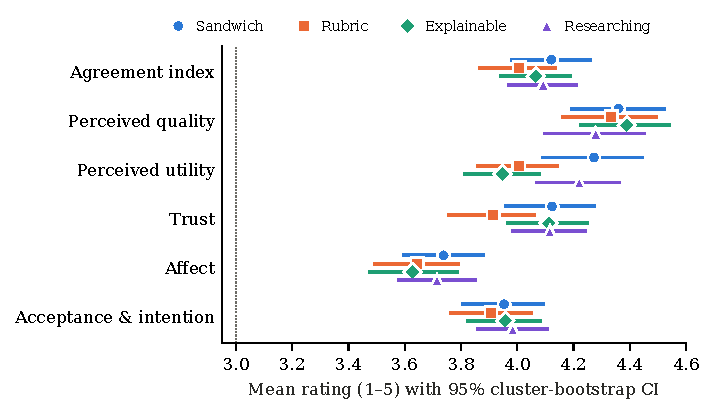
\includegraphics[width=0.85\textwidth]{format_constructs.pdf}
    \Description{A diagram depicting the conceptual constructs and measurement framework used for evaluation.}
    \caption{Overview of the conceptual construct framework and evaluation metrics.}
    \label{fig:framework}
\end{figure}

As shown in Fig.~\ref{fig:framework}, all illustrations must be referenced directly in the text. Captions are set in 9-point font, centered if single-line, and justified if multi-line.

% -------------------------------------------------------------------------
\section{Empirical Evaluation and Survey Design}
\label{sec:experiments}
Describe the experimental setting, participant demographics, questionnaire instrumentation, and procedure.

\subsection{Instrumentation and Construct Measurements}
% Springer Guideline:
% Table captions should ALWAYS appear ABOVE the table.
% Use professional booktabs rules (\toprule, \midrule, \bottomrule).
\begin{table}[htbp]
\centering
\caption{Summary of survey constructs, dimensions, and operational definitions.}
\label{tab:constructs}
\begin{tabular}{llp{7.5cm}}
\toprule
\textbf{Construct} & \textbf{Metric/Code} & \textbf{Operational Definition} \\
\midrule
Accuracy & ACC & Correctness of technical explanations and error diagnoses. \\
Clarity & CLA & Ease of comprehension, structure, and readability. \\
Specificity & SPE & Concrete pointers to lines of code or specific logic. \\
Transparency & TRA & Explainability of why and how the feedback was derived. \\
Actionability & ACT & Practical guidance on how to fix or refine the implementation. \\
Acceptance & ACP & Student agreement and willingness to adopt recommendations. \\
\bottomrule
\end{tabular}
\end{table}

Table~\ref{tab:constructs} highlights the evaluation dimensions. The numbering of tables and figures continues sequentially throughout the manuscript.

% -------------------------------------------------------------------------
\section{Results and Discussion}
\label{sec:results}
Present statistical analyses, survey findings, correlation matrices, and thematic student responses.

\subsection{Analysis of Survey Constructs (RQ1)}
Present findings addressing RQ1. Reference additional figures where necessary:
\begin{figure}[htbp]
    \centering
    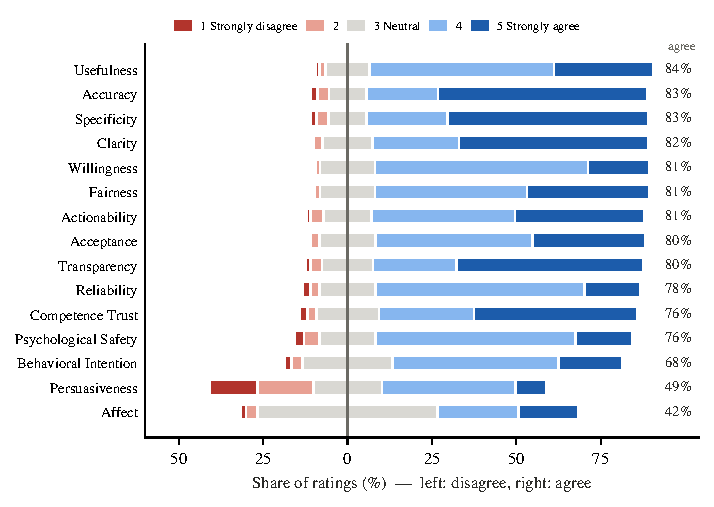
\includegraphics[width=0.85\textwidth]{likert_items.pdf}
    \Description{Distribution of student responses across Likert-scale evaluation items.}
    \caption{Distribution of student responses across the Likert-scale items.}
    \label{fig:likert}
\end{figure}

Fig.~\ref{fig:likert} illustrates the Likert-scale distributions observed in the participant cohort.

\subsection{Cross-Feedback Comparative Analysis (RQ2)}
Examine differences among feedback styles or presentation formats.

\subsection{Source Modality Comparison (RQ3)}
Compare question generation modalities (e.g., codebase extraction vs. knowledge graph).
\begin{figure}[htbp]
    \centering
    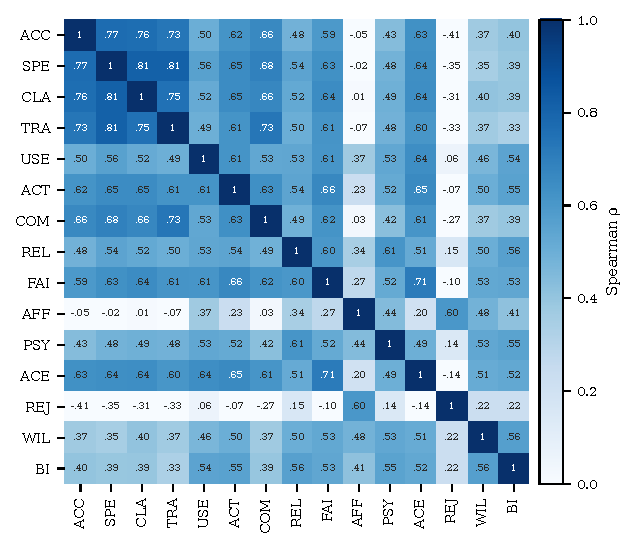
\includegraphics[width=0.85\textwidth]{item_correlations.pdf}
    \Description{Correlation heatmap showing inter-construct relationships among survey items.}
    \caption{Correlation matrix across evaluation dimensions and survey questions.}
    \label{fig:correlations}
\end{figure}

Fig.~\ref{fig:correlations} depicts the inter-item correlation coefficients.

% -------------------------------------------------------------------------
\section{Threats to Validity}
\label{sec:threats}
Discuss construct validity, internal validity, external validity, and reliability considerations.

% -------------------------------------------------------------------------
\section{Conclusion and Future Work}
\label{sec:conclusion}
Summarize the main takeaways, lessons learned, and future research directions.

% =========================================================================
% Back Matter: Credits (Acknowledgements & Disclosure of Interests)
% Springer Guideline: Required placement before Appendix / Bibliography
% =========================================================================
\begin{credits}
\subsubsection{\ackname}
This research was supported by Project Grant Number XYZ. The authors express their gratitude to the student participants and course instructors for their support during data collection.

\subsubsection{\discintname}
The authors have no competing interests to declare that are relevant to the content of this article.
\end{credits}

% =========================================================================
% Appendix (Optional)
% Springer Guideline: If present, place in front of the references.
% =========================================================================
\appendix
\section{Survey Instrument Details}
\label{sec:appendix_survey}
Detailed survey questions and Likert-scale coding schemes can be provided here. Continues the same formatting standards as the main text.

% =========================================================================
% Bibliography
% Springer Guideline:
% Use splncs04.bst style with alphabetic sorting and DOIs for CrossRef.
% =========================================================================
\bibliographystyle{splncs04}
\bibliography{references}

\end{document}

